\documentclass[12pt, a4paper]{report}

%---- GENERAL ---%
\usepackage[utf8x]{inputenc} % Encodage du fichier
\usepackage[T1]{fontenc}  % Encodage des polices du document
\usepackage[english, francais]{babel} % Langages utilisés
\usepackage{lmodern} % Police pour rendre le texte sélectionable

\usepackage[top=2.5cm, bottom=2.5cm, left=2.5cm, right=2.5cm]{geometry} % Marges PDF

%---- TABLE DES MATIERES - PRESENTATION ---%
\usepackage[titles]{tocloft} % Package pour paramtérer la table des matières
\renewcommand{\cftchapleader}{\cftdotfill{\cftdotsep}} % Mets des points pour les chapitre et les sections
\usepackage[colorlinks=true,urlcolor=blue,pdfstartview=FitH,linkcolor=blue,hyperfootnotes=true]{hyperref} % Liens

%---- GLOSSAIRE ---%
\usepackage{glossaries}
\makeglossaries

%---- STRUCTURES DE DONNEES & MISE EN FORME ---%
\usepackage{enumerate} % Listes
\usepackage{graphicx} % Figures
\usepackage{color} % Couleur
\definecolor{darkblue}{RGB}{0,0,190}
\definecolor{lightgray}{gray}{0.70}
\definecolor{darkgreen}{RGB}{0,150,50}

%---- HEADERS & FOOTERS ---%
\usepackage{fancyhdr}
\pagestyle{fancy}
\renewcommand{\sectionmark}[1]{\markright{#1}}
\fancyhf{}

\fancyhead[RE]{\chaptername{} \thechapter{} - \nouppercase{\rightmark}} % Even page - Right side
\fancyhead[LE]{\thepage} % Even page - Left side
\fancyhead[RO]{\thepage}% Odd page - Rigth side
\fancyhead[LO]{\chaptername{} \thechapter{} - \nouppercase{\rightmark}} % Odd page - Left side
\fancyfoot[C]{footer} % Footer - Center

\newcommand{\clearemptydoublepage}{\newpage{\pagestyle{empty}\cleardoublepage}} % Supprime les en-têtes et pieds de page des pages vides (type book)

%---- CHAPTERS ---%
\usepackage[Lenny]{fncychap}

%---- CODES SOURCES & ALGORITHMES ---%
\usepackage{listings} % Codes sources

% [style = sourceC] for the C codes
\lstdefinestyle{sourceC}{language=C, basicstyle=\small\color{black}\ttfamily, classoffset=0, keywordstyle=\color{blue}\bfseries, classoffset=1, morekeywords={NULL}, keywordstyle=\color{magenta}\bfseries, commentstyle=\color{brightblue}\itshape, stringstyle=\color{darkgreen}, showstringspaces=false, tabsize=3, framexleftmargin=2mm, frame=shadowbox, rulesepcolor=\color{lightgray}, breaklines=true, emph={main, printf, scanf, FILE, fopen, fscanf, fprintf, fclose, rand}, emphstyle=\color{darkblue}\bfseries,columns=
fullflexible, flexiblecolumns=true, upquote=true, keepspaces=true}

% [style = inlineSourceC] for C expression into text
\lstdefinestyle{inlineSourceC}{language=C, basicstyle=\footnotesize\color{black}\ttfamily, classoffset=0, keywordstyle=\color{blue}\bfseries, classoffset=1, morekeywords={NULL}, keywordstyle=\color{magenta}\bfseries, commentstyle=\color{brightblue}\itshape, stringstyle=\color{darkgreen}, showstringspaces=false, tabsize=3, breaklines=true, emph={main, printf, scanf, FILE, fopen, fscanf, fprintf, fclose, rand}, emphstyle=\color{darkblue}\bfseries,columns=fullflexible, keepspaces=true,upquote=true}

% [style = sourceJava] for the Java codes
\lstdefinestyle{sourceJava}{language=Java, basicstyle=\small\color{black}\ttfamily, classoffset=0, keywordstyle=\color{darkgreen}\bfseries, commentstyle=\color{brightblue}\itshape, stringstyle=\color{darkgreen}, showstringspaces=false, tabsize=3, framexleftmargin=2mm, frame=shadowbox, rulesepcolor=\color{lightgray}, breaklines=true, emph={main, printf, FILE, fopen, fscanf, fprintf, fclose,new,return,this,super,null,break,continue,if,else,switch,case,default,do,while,for,break,new,return}, emphstyle=\color{darkred}\bfseries,columns=fullflexible,upquote=true}

% [style = sourceJava] for the Java codes
\lstdefinestyle{inlineSourceJava}{style=sourceJava, basicstyle=\normalsize\color{black}\ttfamily}

% [style = msgTerminal] for shell codes on black background
\lstdefinestyle{msgTerminal}{language=sh, basicstyle=\small\color{white}\ttfamily, keywordstyle=\color{white}, commentstyle=\color{white}\itshape, stringstyle=\color{white}, showstringspaces=false, framexleftmargin=3mm, xleftmargin=3mm, frame=none, tabsize=3, backgroundcolor=\color{black}, rulecolor=\color{black}, breaklines=true,columns=fullflexible,upquote=true}

% [style = msgTerminalW] for shell codes on white background
\lstdefinestyle{msgTerminalW}{language=sh, basicstyle=\small\color{black}\ttfamily, keywordstyle=\color{black}, commentstyle=\color{black}\itshape, stringstyle=\color{black}, showstringspaces=false, framexleftmargin=3mm, xleftmargin=3mm, frame=none, tabsize=3, backgroundcolor=\color{white}, rulecolor=\color{white}, breaklines=true,columns=fullflexible,upquote=true}

% [style = inlineTerminal] for shell expression into text
\lstdefinestyle{inlineTerminal}{language=sh, basicstyle=\footnotesize\color{black}\ttfamily\bfseries, keywordstyle=\color{black}, commentstyle=\color{black}\itshape, stringstyle=\color{black}\itshape, showstringspaces=false, tabsize=3, breaklines=true,upquote=true}


\usepackage[french]{algorithm2e} % Algorithmes 
\newenvironment{algo}[0]{\vrule~\vrule\itshape \begin{algorithm}[H] }{\normalfont\end{algorithm}}
\newcommand{\var}[1]{\textnormal{\texttt{#1}}}
\RestyleAlgo{plain}
\SetKwSwitch{Selon}{Cas}{Autre}{selon}{faire}{cas où}{autres cas}{fin}{fin} %Si la compilation bloque à algorithm2e, tenter la ligne du dessous à la place de celle-là
%\SetKwSwitch{Selon}{Cas}{Autre}{selon}{faire}{cas où}{autres cas}{fin}
\SetKwRepeat{Repeter}{r\'ep\'eter}{tant que}
\SetKwFor{uTq}{tant que}{faire}{} % Tant que sans fin (équivaut a uSi)
\SetKwFor{oTq}{}{}{fin} % Tant que déjà ouvert, donc sans balise de depart
\SetKwIF{oSi}{}{}{}{}{}{}{fin}
\SetKwIF{oFn}{}{}{fonction}{}{}{}{fin}
\SetKwFunction{KwFn}{Fn}


%---- DOCUMENT ---%
% COMPILATION : 
% pdflatex squelette_rapport.tex
% bibtex squelette_rapport
% makeindex squelette_rapport
% pdflatex squelette_rapport.tex
% pdflatex squelette_rapport.tex

\title{\textbf{Portage architecture Arduino vers ESP32} \\ \Large{--- Épita --- \\ \textit{Équipe Robotique d'Exploration}} \\ \vspace{1,5cm} 
\includegraphics[width=0.3\textwidth]{./img/logo_epita} 
\includegraphics[width=0.2\textwidth]{./img/logo_equipe_robotique_exploration} \vspace{1,5cm}}
\date{\today}
\author{Tony BERNIS \and Valentin DUMOUSSET \and Julien LE QUANG \and Merlin VOTAT}

\begin{document}
	\maketitle
	
	

	%-----------------------
	\chapter*{Résumé}
	\addcontentsline{toc}{chapter}{Résumé}
	%-----------------------	

Micro ROS (Robot Operating System) est un framework pour faciliter le développement robotique et qui sert d'interface entre les micro controleurs.
Il permet ainsi l'abstraction du matériel, la transmission de message etc.
Micro ROS n'est pas disponible sur toutes les cartes Arduino. Dans notre projet, nous avons choisi une carte Nano RP2040.
L'objectif de notre projet est dans un premier temps de faire bouger l'arraignée et dans un second temps travailler sur la synchronisation entre une autre arraignée.

Exemple gras et italique~:

Sed ut \textbf{perspiciatis} unde omnis iste \textbf{natus} error sit voluptatem accusantium doloremque laudantium, totam rem aperiam, eaque ipsa quae ab illo inventore \textit{veritatis} et quasi architecto beatae vitae dicta sunt explicabo. Nemo enim ipsam voluptatem quia voluptas sit aspernatur aut odit aut fugit, sed quia consequuntur magni dolores eos qui ratione voluptatem sequi nesciunt. Neque porro quisquam est, qui dolorem ipsum quia dolor sit amet, consectetur, adipisci velit, sed quia non \textit{numquam eius modi tempora incidunt ut} labore et dolore magnam aliquam quaerat voluptatem. \textbf{Ut enim ad minima veniam, \textit{quis nostrum} exercitationem ullam corporis} suscipit laboriosam, nisi ut aliquid ex ea commodi consequatur? 

Exemple texte centré~:

\begin{center}
	Quis autem vel eum iure reprehenderit qui in ea voluptate velit esse quam nihil molestiae consequatur, vel illum qui dolorem eum fugiat quo voluptas nulla pariatur? Nemo enim ipsam voluptatem quia voluptas sit aspernatur aut odit aut fugit, sed quia consequuntur magni dolores eos qui ratione voluptatem sequi nesciunt.
\end{center}

Ut enim ad minim veniam, \color{green} quis nostrud exercitation ullamco \color{black} laboris nisi ut aliquip ex ea commodo consequat. Duis aute irure dolor in reprehenderit in voluptate velit esse cillum dolore eu fugiat nulla pariatur. Excepteur sint occaecat cupidatat non \color{darkblue} proident, sunt in culpa \color{black} qui officia deserunt mollit anim id est laborum.
	
	%-----------------------
	% TABLE DES MATIERES %
	\tableofcontents
	%-----------------------

	%-----------------------%
	%     INTRODUCTION      %
	%-----------------------%
	
	%-----------------------
	\chapter{Introduction}
	%-----------------------

ROS2 (Robot Operating System) est un système d'exploitation open source pour les robots. 
Il est conçu pour faciliter le développement de logiciels pour les robots en offrant des bibliothèques, 
des outils et des standards communs pour la robotique. ROS2 offre une infrastructure logicielle pour la programmation de robots, 
y compris des fonctionnalités telles que la communication entre les composants logiciels, la gestion des données, 
la planification et l'exécution de tâches, la visualisation de données, et bien plus encore. 
ROS2 est utilisé dans de nombreux types de robots, des petits robots de service aux grands robots industriels. 
\linebreak

Micro-ROS est une version légère de ROS2 conçue pour fonctionner sur des systèmes embarqués avec 
des ressources limitées en termes de calcul et de mémoire. Micro-ROS offre une infrastructure logicielle pour la programmation 
de robots embarqués, y compris des fonctionnalités similaires à celles de ROS2, telles que la communication entre les composants 
logiciels, la gestion des données, la planification et l'exécution de tâches. 
Micro-ROS est conçu pour être facile à utiliser et à intégrer dans des projets de robotique embarqué, en offrant une grande 
flexibilité et une grande efficacité en termes de ressources. 
\linebreak

Le but de notre projet était d’explorer les différentes options qui nous permettraient d’adapter le code des araignées 
mécaniques sur l’architecture Micro-Ros. 
\linebreak

Il y a plusieurs avantages à utiliser Micro-ROS pour programmer une araignée mécanique. 
Tout d'abord, Micro-ROS est conçu pour fonctionner sur des systèmes embarqués avec des ressources limitées en termes 
de calcul et de mémoire, ce qui est idéal pour une araignée mécanique qui a des contraintes en termes de taille et de poids. 
En outre, Micro-ROS offre une infrastructure logicielle pour la programmation de robots. 
Enfin, Micro-ROS est une version légère de ROS2, ce qui signifie qu'il est moins gourmand en ressources que ROS2 tout en offrant 
les mêmes fonctionnalités de base. Cela peut améliorer les performances de l'araignée mécanique en utilisant moins de ressources 
pour exécuter le logiciel. 
\linebreak

Dans ce rapport, nous allons présenter toutes les recherches que nous avons effectué pendant ce projet, les différentes 
solutions que nous avons conceptualisées ainsi que la solution que nous avons choisie et sa mise en œuvre. 
\linebreak


	%-----------------------%
	%    ETAT DE L'ART      %
	%-----------------------%

	%-----------------------
	\chapter{État de l'Art}
	\thispagestyle{empty}
	%-----------------------

		%-----------------------
		\section{Les solutions}
		%-----------------------

			%-----------------------
			\subsection{Solution 1}
			%-----------------------

A l’heure actuelle, Micro-ros n’est supporté que par 2 modèles de cartes Arduino, Arduino Portenta H7 M7 Core
\url{https://store.arduino.cc/portenta-h7} et Arduino Nano RP2040 Connect \url{https://docs.arduino.cc/hardware/nano-rp2040-connect}. 

Nous avons d'ailleurs vu qu'une personne a installé Micro ROS sur ces cartes : \url{https://www.youtube.com/watch?v=mq1uFGsYqeU}.

Il était probablement possible d’adapter Micro-ROS à la carte Arduino que nous avions à notre disposition mais cela risquait de nous 
prendre plus de temps que nous n’avions à disposition.  
\linebreak
	
L'Arduino Nano RP2040 Connect est une carte de développement basée sur le processeur ARM Cortex-M0+ RP2040 conçue par Raspberry Pi. 
Elle est conçue pour être petite, flexible et facile à utiliser pour les projets de robotique et d'Internet des objets (IoT). 
L'Arduino Nano RP2040 Connect est équipée de 20 broches de E/S numériques, de 6 broches PWM, de 6 broches analogiques, 
d'un port USB-C pour l'alimentation et la communication, d'un connecteur de batterie, d'un connecteur de microphone, 
d'un connecteur de haut-parleur et d'un connecteur de bouton-poussoir. La carte est également compatible avec les bibliothèques Arduino 
pour faciliter le développement de logiciels pour les projets de robotique et d'IoT. 
Après nos différentes recherches, nous avons conclu que ce serait la carte idéale pour mettre en place le projet.
\linebreak 

\begin{figure}[H]
\begin{center}
	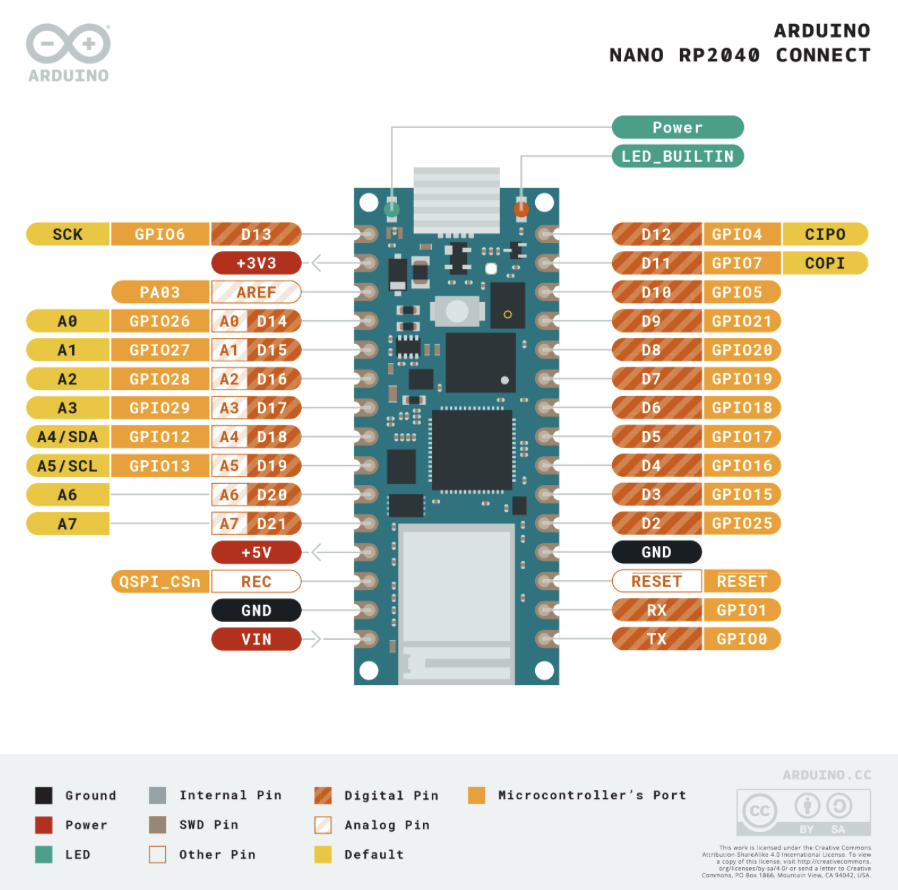
\includegraphics[width=0.7\textwidth]{./img/schema_carte_1}
\end{center}
\end{figure}

\begin{figure}[H]
\begin{center}
	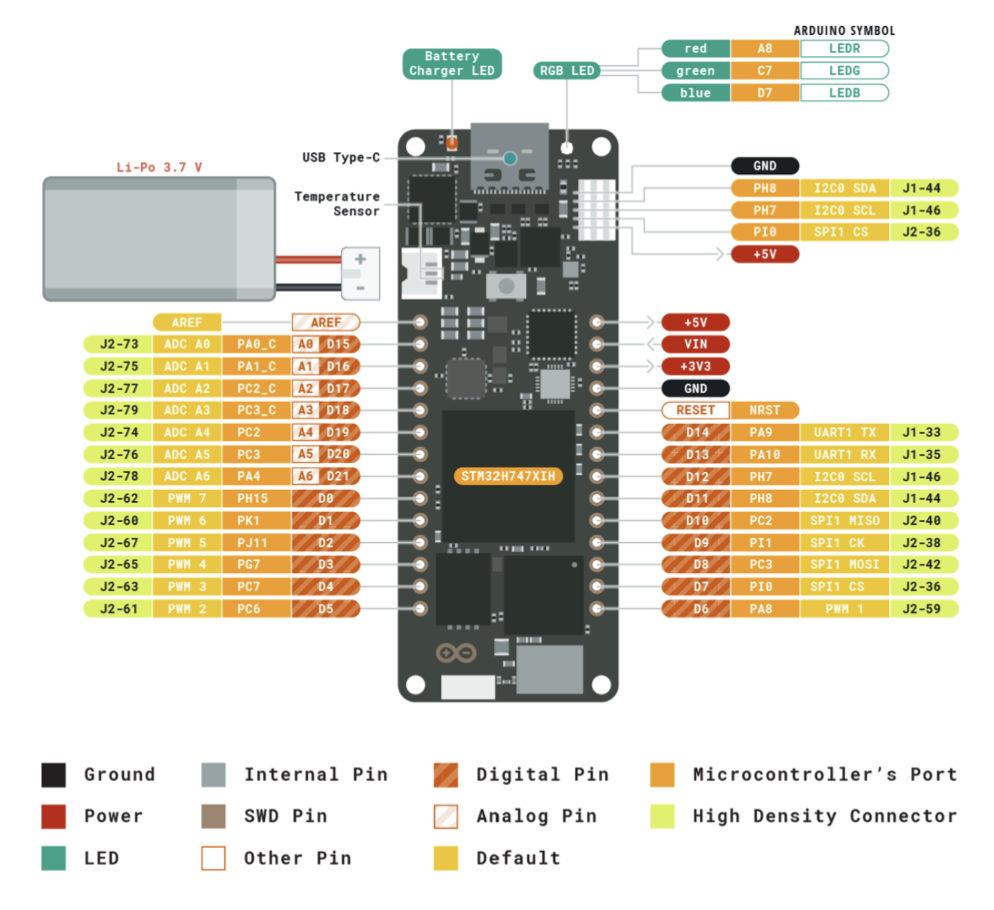
\includegraphics[width=0.7\textwidth]{./img/schema_carte_2}
\end{center}
\end{figure}

			%-----------------------
			\subsection{Solution 2}
			%-----------------------

Nous avons cependant pensé à une solution alternative. Nous pouvons aussi utiliser une carte ESP32 qui est déjà compatible 
avec l’architecture Micro-ROS ( \url{https://micro.ros.org/blog/2020/08/27/esp32} ).  
\linebreak

ESP32 est une puce de microcontrôleur à double cœur conçue par Espressif Systems. Elle est principalement utilisée 
dans les applications de robotique, d'Internet des objets (IoT) et de réseaux locaux sans fil (Wi-Fi et Bluetooth). 
La puce ESP32 est équipée d'un processeur principal Xtensa Dual-Core LX6, d'un processeur coprocesseur ultra-basse consommation, 
d'une mémoire SRAM de 520 Ko, d'une mémoire flash de 16 Mo, d'un module Wi-Fi 802.11b/g/n/e/i et d'un module Bluetooth v4.2. 
La puce ESP32 offre également de nombreux E/S numériques, analogiques et PWM, ainsi que des fonctionnalités avancées telles 
que le traitement du signal numérique, le traitement en temps réel, l'interface de caméra et l'interface de bus série. 
En raison de ses performances et de ses fonctionnalités avancées, la puce ESP32 est largement utilisée dans de nombreux projets de 
robotique et d'IoT.
\linebreak
	
On peut installer cette carte sur notre robot et la brancher directement en SPI (Serial Peripheral Interface) avec la carte Arduino Nano pour 
ne pas avoir à la connecter en radio ou en wifi.  
L’ESP32 s’occupera de faire tous les contrôles et enverra des ordres à la carte Arduino qui se contentera de les exécuter; 
Les problèmes que l’on pourrait rencontrer avec cette méthode sont le manque de place sur le robot, un poids peut-être trop important, ainsi 
qu’un manque d’alimention, l’alimentation actuelle du robot ne sera peut-être pas suffisante pour alimenter les deux cartes. 
\linebreak

		%-----------------------
		\section{Installation de ROS 2}
		%-----------------------

Nous allons détailler dans cette section comment installer ROS 2 sur Linux et Windows.
\linebreak

\underline{Sur Linux (Recommandé) :}
 
Suivre la documentation suivante :
\url{https://docs.ros.org/en/rolling/Installation/Ubuntu-Install-Debians.html}
 \linebreak

 \underline{Sur Windows :}
 
 \begin{enumerate}
	\item Téléchargez la dernière version de ROS2 depuis le site Web officiel de ROS (\url{https://index.ros.org/doc/ros2/}). 
	Sélectionnez la version de ROS2 qui convient à votre version de Windows (32 bits ou 64 bits). 

	\item Installez les outils de build Colcon en suivant les instructions du site Web de ROS 
	(\url{https://index.ros.org/doc/ros2/Installation/Colcon/}).
	Colcon est un outil de build utilisé pour compiler et intégrer les logiciels ROS2. 

	\item Créez un environnement de développement ROS2 en utilisant l'outil "ament" 
	(\url{https://index.ros.org/doc/ros2/Installation/Ament/}).
	Ament est un outil qui permet de gérer les dépendances et les environnements de développement pour les projets ROS2. 

	\item Installez les bibliothèques de support de Windows pour ROS2 en suivant les instructions du site Web de ROS 
	(\url{https://index.ros.org/doc/ros2/Installation/Windows-Support/}).
	Ces bibliothèques sont nécessaires pour exécuter ROS2 sur Windows. 

	\item Ajoutez les variables d'environnement ROS2 à votre système en suivant les instructions du site Web de ROS 
	(\url{https://index.ros.org/doc/ros2/Installation/Windows-Environment-Variables/}).
	Ces variables d'environnement sont nécessaires pour exécuter les commandes ROS2 et accéder aux outils et aux bibliothèques ROS2 
	depuis n'importe quel emplacement de votre système. 

	\item Vérifiez que ROS2 est correctement installé en exécutant la commande "ros2 run demo\_nodes\_cpp talker" depuis une 
	invite de commandes.
	Cette commande devrait exécuter un noeud "talker" de démonstration qui envoie des messages de test à un noeud "listener" de démonstration.
	Si la commande s'exécute correctement, cela signifie que ROS2 est correctement installé et configuré sur votre système.

	\item Vous pouvez maintenant commencer à développer vos propres applications ROS2 en suivant les tutoriels et les exemples disponibles 
	sur le site Web de ROS (\url{https://index.ros.org/doc/ros2/}).
	N'oubliez pas de configurer votre environnement de développement et de compiler vos logiciels avec Colcon avant de les exécuter.
\end{enumerate}

L'étape suivante est de générer l'agent Micro ROS et le lancer. On peut retrouver à cet effet un tutoriel à cette adresse :
\url{https://gist.github.com/Redstone-RM/0ca459c32ec5ead8700284ff56a136f7}
\linebreak

\clearemptydoublepage


			
	%-----------------------%
	% ETUDE DE FAISABILITE  %
	%-----------------------%

	%-----------------------
	\chapter{Implémentation}
	%-----------------------

Introduction de l'étude de faisabilité - Lorem ipsum dolor sit amet, consectetur adipisicing elit, sed do eiusmod tempor incididunt ut labore et dolore magna aliqua. Ut enim ad minim veniam, quis nostrud exercitation ullamco laboris nisi ut aliquip ex ea commodo consequat. Duis aute irure dolor in reprehenderit in voluptate velit esse cillum dolore eu fugiat nulla pariatur. Excepteur sint occaecat cupidatat non proident, sunt in culpa qui officia deserunt mollit anim id est laborum.

	Sed ut perspiciatis unde omnis iste natus error sit voluptatem accusantium doloremque laudantium, totam rem aperiam, eaque ipsa quae ab illo inventore veritatis et quasi architecto beatae vitae dicta sunt explicabo. Nemo enim ipsam voluptatem quia voluptas sit aspernatur aut odit aut fugit, sed quia consequuntur magni dolores eos qui ratione voluptatem sequi nesciunt. Neque porro quisquam est, qui dolorem ipsum quia dolor sit amet, consectetur, adipisci velit, sed quia non numquam eius modi tempora incidunt ut labore et dolore magnam aliquam quaerat voluptatem.
	
		%-----------------------
		\section{Implémentation technique}
		%-----------------------

// A confirmer / compléter par notre expert Merlin

			%-----------------------
			\subsection{Les différences entre ROS et ROS2}
			%-----------------------

Une des principales différences entre ROS et ROS2 est leur architecture. ROS est basé sur une architecture monolithique, 
dans laquelle tous les composants logiciels sont intégrés dans un seul et même système d'exploitation. 
ROS2, en revanche, est basé sur une architecture modulaire, dans laquelle chaque composant logiciel peut être exécuté 
indépendamment des autres dans un système d'exploitation distribué. Cette architecture modulaire permet une meilleure flexibilité, 
une meilleure évolutivité et une meilleure tolérance aux pannes que l'architecture monolithique de ROS. 
\linebreak

Une autre différence importante entre ROS et ROS2 est leur modèle de communication. ROS utilise un modèle de communication basé 
sur le publisheur-abonné, dans lequel les composants logiciels peuvent envoyer et recevoir des données en utilisant des "topics" définis. 
ROS2, en revanche, utilise un modèle de communication basé sur les services et les requêtes, dans lequel les composants logiciels peuvent 
interagir en invoquant des services et en envoyant des requêtes. Ce modèle de communication permet une meilleure gestion des données et 
une meilleure flexibilité pour les applications de robotique. 
\linebreak

Enfin, ROS et ROS2 diffèrent également en termes de langages de programmation et de plateformes de développement. 
ROS prend en charge principalement le langage de programmation C++, bien qu'il soit également possible de l'utiliser avec d'autres 
langages tels que Python. ROS2 prend en charge plusieurs langages de programmation, tels que C++, Python, Java, et bien d'autres. 
De plus, ROS utilise principalement le système de build Catkin pour la compilation et l'intégration de logiciels, alors que 
ROS2 utilise l'outil de buildmentament Colcon. 

		%-----------------------
		\section{Limites et problèmes rencontrés}
		%-----------------------

			%-----------------------
			\subsection{Limites}
			%-----------------------

Alimentation : cartes besoin d'une batterie externe supplémentaire 

Nous avons pensé à faire un support mais nous n'avons pas eu le temps (le support n'étant pas un élément essentiel).

Soucis de compatibilité sur différents OS :  
\begin{itemize}
	\item[$\bullet$] sur Mac, il y avait un problème de dépendance python (graphviz) bien que la dépendance était installée
	\item[$\bullet$]sur Ubuntu 18.04, le framework ne fonctionnait pas (problème pour afficher une fenêtre graphique)
\end{itemize}

Il existe plusieurs versions de ROS, chacune étant destinée pour une version Linux spécifique. 
La dernière est la version humble et qui est compatible avec la version 22.04 d’Ubuntu.  
On retrouvera la documentation à cette adresse : \url{https://docs.ros.org/en/humble/Installation/Ubuntu-Install-Debians.html}
On peut également utiliser une image Docker pour ROS 2. 
\linebreak
Nous avons utilisé l’IDE Platform IO qui est une extension de VS Code. 
Il est compatible Windows, Mac et Linux. L’étape suivante était de générer l’agent Micro-ROS et le lancer.  
Nous avons testé la connexion wifi entre l’agent sur l’ordinateur et la carte en utilisant le code exemple de la libraire micro-ROS : 
(\url{https://github.com/micro-ROS/micro_ros_arduino/blob/galactic/examples/micro-ros_publisher_wifi/micro-ros_publisher_wifi.ino}) 
L’exemple initie la connexion wifi et envoie un message à la carte. Lorsque la connexion wifi échoue, la diode sur la carte se 
met à clignoter de manière intempestive. Nous avons testé ensuite le code de l’araignée SEALK pour tester les mouvements mais le code 
fourni ne marchait pas sur la carte. En effet, nous avions le problème de compilation suivant :  

\begin{lstlisting}
src/armcontroller.h:52:13: error: there are no arguments to 'sei' 
that depend on a template parameter, so a declaration of 'sei' 
must be available [-fpermissive]
sei();
\end{lstlisting}
Cette interruption permet d'activer les interruptions de timer.

			%-----------------------
			\subsection{Problèmes rencontrés}
			%-----------------------

Servomoteur : on a besoin de la lib RP2040\_ISR\_Servo (\url{https://github.com/khoih-prog/RP2040_ISR_Servo}) car les mouvements envoient une instruction en dehors de la loop principale

Impossible d'utiliser l'Arduino IDE (car il manque un time.h).

Nous avons utilisé VSCode avec PlatformIO qui est une extension de VSCode. Il est compatible Windows, Mac et Linux.

PlatformIO est designé pour faire marcher énormément de cartes et il faut donc spécifier la carte sur laquelle on travaille. Il se charge ensuite de récupèrer les libs.




	%-----------------------%
	%       CONCLUSION      %
	%-----------------------%
	
	%-----------------------
	\chapter{Conclusion}
	%-----------------------

Conclusion du document - En conclusion, notre projet d'exploration informatique a permis de découvrir de nouvelles technologies, 
méthodes et outils dans le domaine de l'informatique. Nous avons évalué les différentes approches et technologies disponibles, 
et avons choisi celles qui nous semblaient les plus adaptées à notre projet. Nous avons mis en œuvre notre solution en utilisant 
les technologies et les outils sélectionnés, et avons obtenu réussi a atteindre nos objectifs (nous avons réussi à mettre en mouvement 
les araignées et à les synchroniser). 
En plus de nos résultats techniques, ce projet a également été bénéfique pour notre cursus en informatique. 
Nous avons eu l'occasion de mettre en pratique les connaissances et les compétences que nous avons acquises au cours de nos études, 
et d'en apprendre de nouvelles. Nous avons également développé des compétences en matière de travail en équipe, de communication, 
de gestion de projet et de résolution de problèmes. Ce projet a été une expérience précieuse pour notre formation en informatique 
et nous espérons qu'il nous aidera à poursuivre notre carrière dans ce domaine passionnant. 
Nous avons également identifié les limites de notre solution et avons défini les directions futures pour la recherche et le 
développement dans ce domaine. En somme, ce projet d'exploration informatique a été une expérience enrichissante et nous espérons 
qu'il contribuera à l'avancement de l'informatique. 

\newglossaryentry{word1}{name=mot en entier, description={Définition du mot}}
\newglossaryentry{word2}{name=anotherword, description={Bla bla}}

Voici une phrase qui utilise un \gls{word1} du glossaire et encore un autre \gls{word2}.
	

	%-----------------------%
	%      GLOSSAIRE        %
	%-----------------------%
	%-----------------------
	\chapter*{\centerline{\MakeUppercase{Glossaire}}}
	%-----------------------


\begin{itemize}
	\item[$\bullet$] Ros2 : ROS2 (Robot Operating System 2) est un système d'exploitation open source pour les robots, 
    basé sur une architecture modulaire et un modèle de communication basé sur les services et les requêtes, qui permet de 
    développer et d'exécuter des applications de robotique de manière flexible et scalable. 

    \item[$\bullet$] Micro-ROS : Micro-ROS est une implémentation légère de ROS2 (Robot Operating System 2) conçue pour être 
    exécutée sur des périphériques embarqués tels que les microcontrôleurs et les cartes de développement. 
 
    \item[$\bullet$] Esp32 : ESP32 est un microcontrôleur de la famille ESP de Espressif Systems, conçu pour être utilisé 
    dans des applications embarquées telles que les objets connectés et les capteurs. 
     
    \item[$\bullet$] Arduino Nano : Arduino Nano est une carte de développement microcontrôleur basée sur un microcontrôleur Atmel AVR. 
    Elle est conçue pour être petite et portable, avec un format de circuit imprimé compact qui peut être facilement intégré dans des 
    projets de robotique et d'objets connectés. 
     
    \item[$\bullet$] OpenSCAD : OpenSCAD est un logiciel de modélisation 3D de type "constructif", qui permet de créer des modèles 3D 
    en utilisant une syntaxe de script plutôt que par une interface graphique. 
\end{itemize}
% K.O?
%\deftranslation{Glossary}{Glossaire}
%\addcontentsline{toc}{chapter}{Glossaire} % Rajoute la partie dans le sommaire
%\printglossaries
	
	%-----------------------%
	%      BIBLIOGRAPHIE    %
	%-----------------------%

\addcontentsline{toc}{chapter}{Bibliographie} % Rajoute la partie dans le sommaire
\bibliographystyle{alpha}
\bibliography{biblio/bibliographie.bib}

	
\end{document}